%!TEX root=ClassNotes.tex
\section{Limits \& Continuity}

We'll now use the proof techniques we've learned so far to study functions.

We'll start with rigorously defining limits. At first this might seem unnecessarily complicated, but having precise definitions will allow us to make more and more sophisticated constructions and later on in the course enable us to prove statements about derivatives and integrals.

Time permitting, towards the end of the semester, we'll construct the Weierstrass function, a function defined on real numbers which is continuous everywhere but differentiable nowhere! But it all starts with the definition of a limit.

\begin{figure}[H]
	\centering
	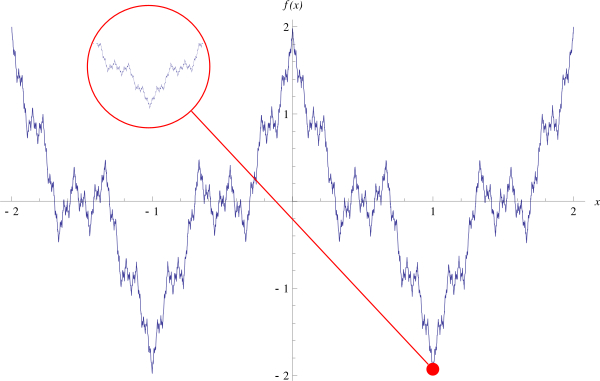
\includegraphics[width=0.6\textwidth]{WeierstrassFunction.jpg}
	% \captionsetup{labelformat=empty}
	\caption*{Weierstrass function (Image from Wikipedia)}
\end{figure}

\subsection{Limits}
At the heart of all analysis (and hence calculus) lies the notion of a limit. Almost every single concept that we'll define will be a limit of some kind.

\begin{definition}[Provisional definition of limit]
	\label{def:provisional_definition_limit}
	For a function $f$ and a real number $a$, we say that the function $f$ \textbf{approaches a limit $L$ at $a$}, for some real number $L$, if we can make $f(x)$ as close to $L$ as we like by requiring that $x$ be sufficiently close to, but unequal to, $a$. This is denoted
	\begin{align*}
		\lim \limits _ {x \rightarrow a} f(x) = L
	\end{align*}
\end{definition}
\noindent There are 3 problems with this definition:
\begin{enumerate}
	\item The terms {\it ``as close to $L$ as we like''} and {\it``sufficiently close''} are not precise. (How close is sufficiently close?)
	\item The order of implication is unclear.
	\item The definition does not give us a way to come up with the limit $L$.
\end{enumerate}

First, we'll make the terms precise.  We can measure the distance between two real numbers $x$, $y$ by taking their difference $x - y$, however, the difference can be negative so we use the absolute value $|x - y|$ instead.  So that
\begin{center}
	\begin{tabular}{l l l}
		{\it $x$ sufficiently close to, but unequal to, $a$} & translates to & {\it $0 < |x - a| < \delta$}                            \\
		{\it $f(x)$ as close to $L$ as we like}              & translates to & {\it for every $\epsilon > 0$, $|f(x) - L| < \epsilon$}\end{tabular}
\end{center}
and the definition of limit becomes\\
\begin{indentPara}
	\dots $f$ \textbf{approaches a limit $L$ at $a$}, for some real number $L$, if we can make $|f(x) - L| < \epsilon$ for every $\epsilon > 0$ by requiring that $0 < |x - a | < \delta$ for some $\delta > 0$.\\
\end{indentPara}

Next, to clarify the order of implication we rephrase the statement in the more standard {\it ``If ... then''} form and put all the quantifiers in the front,\\
\begin{indentPara}
	\dots $f$ \textbf{approaches a limit $L$ at $a$}, for some real number $L$, if for every $\epsilon > 0$, there exists a $\delta > 0$ such that, for all $x$, if $0 < |x - a | < \delta$ then $|f(x) - L| < \epsilon$.\\
\end{indentPara}


The third problem cannot be fixed! There is no systematic way of finding the limit of a general function, the only thing we can do is {\it guess} the limit and then use the definition to {\it prove} that it is indeed the limit. For special functions like polynomials, trig functions, exponential, and logarithms, we can find limits explicitly, which is what makes these functions useful for approximating and estimating more complicated functions.

\begin{definition}[Formal definition of limit]
	\label{def:formal_definition_limit}
	We say that the function $f$ \textbf{approaches a limit $L$ at $a$}, for some real number $L$, if for every $\epsilon > 0$, there exists a $\delta > 0$ such that, for all $x$, if $0 < |x - a | < \delta$ then $|f(x) - L| < \epsilon$.
\end{definition}

\begin{exercise}
	Come up with formal definitions for the following:
	\begin{enumerate}
		\item The function $f$ approaches a limit $L$ at $a$ {\bf from the right}, for some real number $L$, if we can make $f(x)$ as close to $L$ as we like by requiring that $x$ be sufficiently close to, but strictly greater than $a$. This is denoted
		      \begin{align*}
			      \lim \limits _ {x \rightarrow a^+} f(x) = L.
		      \end{align*}
		\item The function $f$ approaches a limit $L$ at $a$ {\bf from the left}, for some real number $L$, if we can make $f(x)$ as close to $L$ as we like by requiring that $x$ be sufficiently close to, but strictly smaller than $a$. This is denoted
		      \begin{align*}
			      \lim \limits _ {x \rightarrow a^-} f(x) = L.
		      \end{align*}
		\item The function $f$ \textbf{approaches the limit $\infty$ at $a$}, if $f(x)$ can be made as large as we like by requiring that $x$ be sufficiently close to, but unequal to, $a$. This is denoted \footnote{
		In mathematics $\infty$ means several things, in fact, there are infinitely many infinities. For us, $\infty$ is a {\it placeholder} for a limit of a function that grows very large. $\infty$ is not a real number and hence cannot be used in equations.}
		      \begin{align*}
			      \lim \limits _ {x \rightarrow a} f(x) = \infty.
		      \end{align*}

		\item The function $f$ \textbf{approaches a limit $L$ at $\infty$}, for some real number $L$ if we can make $f(x)$ as close to $L$ as we like by requiring that $x$ be sufficiently large. This is denoted
		      \begin{align*}
			      \lim \limits _ {x \rightarrow \infty} f(x) = L.
		      \end{align*}
		% \item The function $f$ \textbf{does not approaches a limit $L$ at $a$}. Further generalize this to: the function $f$ does not approaches a limit $L$ at $a$, {\it for any $L$}. In this case, we say that the {\bf limit of $f$ at $a$ does not exist}.
	\end{enumerate}
\end{exercise}

\begin{exercise}
	For each of the following, first guess the limit, then use the formal definition of limit to prove that it is indeed the limit.
	\begin{enumerate}
		\item $\lim \limits_{x \rightarrow 1^+} 2x + 1$
		\item $\lim \limits_{x \rightarrow 1^+} x^2$
		\item $\lim \limits_{x \rightarrow \infty} x^{10} + x$
		\item $\lim \limits_{x \rightarrow 0^+} 1/x$
		% \item $\lim \limits_{x \rightarrow 0^+} \dfrac{\sin x}{x}\qquad$  (You can assume that $\sin x < x - \dfrac{x^3}{6}$ for all $0 < x < 1$.)
		\item $\lim \limits_{x \rightarrow 0} f(x)$ where $f(x) = \begin{cases}
				      x & \mbox{ if $x$ is rational}   \\
				      0 & \mbox{ if $x$ is irrational}
			      \end{cases}$
	\end{enumerate}
\end{exercise}

\subsubsection*{Optional Problems}

\begin{exercise} Give examples to show that the following definitions of $\lim \limits _ {x \rightarrow a} f(x) = L$ are not correct.
	\begin{enumerate}
		\item For every $ \delta > 0$, there exists an $ \epsilon > 0$ such that, for all $x$, if $ 0<|x-a|< \delta$ then $ |f(x) - L|< \epsilon$.
		\item For every $\epsilon > 0$, there exists a $\delta > 0$ such that, for all $x$, if $|f(x) - L| < \epsilon$ then $0 < |x - a| < \delta$.
	\end{enumerate}
\end{exercise}

\begin{exercise}
	Prove that if $\lim \limits _ {x \rightarrow a} f(x) = L$ and $ L \neq 0$ then $\lim \limits _ {x \rightarrow a} 1/f(x) = 1/L$ .
\end{exercise}



\subsubsection{Triangle Inequality}

To prove abstract theorems involving absolute values we will need the following very important inequality called the {\bf triangle inequality}.
\begin{align*}
	|x - y| \le |x| + |y|
\end{align*}
If you think of the points $0$, $x$, $y$ (on the real axis) as being the three vertices of a (degenerate) triangle, then $|x|$, $|y|$, and $|x - y|$ are the lengths of the three sides and the triangle inequality is saying that: {\it the sum of the lengths of two sides of a triangle is greater than or equal to the length of the third side.}\\\\
There are other forms in which the triangle inequality is commonly used, e.g.
\begin{align*}
	|x + y|       & \le |x| + |y|   \\
	|x + y| - |y| & \le |x|         \\
	|x|           & \le |x-y| + |y|
\end{align*}
These inequalities are central to a lot of analysis proofs.

\begin{exercise}$ $
	\begin{enumerate}
		\item Prove that $|x| + |x - 1| \ge 1$ for any real number $x$.
		\item Prove that for any real number $x$, at least one of $|x|$ and $|x-1|$ is $\ge 1/2$.\hint{Proof by Contradiction.}
	\end{enumerate}
\end{exercise}

We'll use these to prove inequalities about the non-existence of limits.

\begin{definition}
	If $f$ does not approach the limit $L$, for any real number or $\infty$ or $-\infty$, then we say that the limit of $f$ at $a$ {\bf does not exist}.
\end{definition}

\begin{exercise}
	\label{q:formal_definition_non_existence_limit}
	Negate the formal definitions of limits and come up with an $\epsilon, \delta$ definition for the following.
	\begin{enumerate}
		\item $f$ {\bf does not} approach the limit $L$, where $L$ is a real number, at $a$.
		\item $f$ {\bf does not} approach the limit $\infty$ at $a$. (Similarly for $-\infty$.)
	\end{enumerate}
\end{exercise}

\begin{exercise}
	\label{q:rational_irrational_discontinuity}
	Let $
		f(x) = \begin{cases}
			1 & \mbox{if $x$ is rational,}   \\
			0 & \mbox{if $x$ is irrational.}
		\end{cases}
	$
	\begin{enumerate}
		\item Prove that for every real number $L$, $\lim \limits_{x \rightarrow 0} f(x) \neq L$.
		\item Prove that $\lim \limits_{x \rightarrow 0} f(x) \neq \infty$. (Similarly for $-\infty$.)
	\end{enumerate}
	Hence the limit of $f$ at $0$ does not exist.
\end{exercise}

\begin{exercise}$ $
	\begin{enumerate}
		\item Prove that $\lim \limits_{x \rightarrow a} f(x) = L$ if and only if $\lim \limits_{x \rightarrow a^+} f(x) = L$ and $\lim \limits_{x \rightarrow a^-} f(x) = L$.\hint{This is very easy, don't overthink! Simply write down the formal definitions.}
		      (Similarly for $\infty$, $-\infty$.)

		\item Prove that $\lim \limits_{x \rightarrow 0} \dfrac{1}{x}$ does not exist.
	\end{enumerate}
\end{exercise}


\subsection{Non-existence of limits}

Let's move backwards and try and understand what it means {\it intuitively} for a function to not approach a limit $L$ near $a$. The solution to Exercise \ref{q:formal_definition_non_existence_limit} is the following:\\

\begin{indentPara}
	{\it (Formal definition)} The function $f$ \textbf{does not approach thelimit $L$ at $a$} if there exists an $\epsilon > 0$, such that for all $\delta > 0$, there exists an $x$ such that, $0 < |x - a | < \delta$ and $|f(x) - L| \ge \epsilon$.\\
\end{indentPara}

Going back to how to we came up with the Formal Definition of Limit 	\ref{def:formal_definition_limit}
from the Provisional Definition of Limit \ref{def:provisional_definition_limit} and replacing the absolute values by the distance between points, we can work backwards and get the following provisional definition:\\

\begin{indentPara}
	{\it (Provisional definition)}
	The function $f$ \textbf{does not approach the limit $L$ at $a$} if no matter how close we are to $a$, there is some $x$ for which $f(x)$ is not close to $L$.
\end{indentPara}


% \subsubsection*{Optional Problems}
% \begin{exercise} $ $
% 	\begin{enumerate}
% 		\item Explain how the provisional definition captures the notion of the failure of the function to approach a limit $L$ at $a$.
% 		\item Starting from the provisional definition try to systematically come up with the formal definition using arguments similar to the ones we made to go from Definition  \ref{def:provisional_definition_limit} to Definition \ref{def:formal_definition_limit}.
% 	\end{enumerate}
% \end{exercise}
%
% \begin{exercise}
% 	It is easy to show that for the function
% 	\begin{align*}
% 		f(x) = \begin{cases}
% 			0 & \mbox{if } x \le 0 \\
% 			1 & \mbox{if } x > 0
% 		\end{cases}
% 	\end{align*}
% 	the limit $\lim \limits_{x \rightarrow 0} f(x)$ does not exist by computing the limits from the left and the right.
%
% 	Try to prove that, $\lim \limits_{x \rightarrow 0} f(x) \neq L$ for some real numbers, say $L = 0$, 1, 1/2, and more generally for any real number, using the formal definition and try to explain what the variables $\epsilon$, $\delta$, $x$ in your proof mean {\it geometrically}.
% \end{exercise}

\subsection{Continuity}

\begin{definition}
  We say that a function $f$ is {\bf continuous} at $a$ if
  \begin{align*}
    \lim \limits_{x \rightarrow a} f(x) = f(a)
  \end{align*}
  We say that a function $f$ is {\bf continuous on an interval} $(a,b)$ it $f$ is continuous at every $x$ in $(a,b)$. \footnote{If we use closed intervals $[a,b]$ instead, then we have to use $\lim \limits_{x \rightarrow a^+}$ and $\lim \limits_{x \rightarrow b^-}$ in the definition of continuity.}
\end{definition}

Thus continuous functions have {nice} limits. Further, we have the following theorem which makes continuous functions easy to manipulate.

\begin{theorem}
  \label{theorem:continuous_functions}
  If the functions $f$, $g$ are continuous at $x=a$ then so are the functions
  \begin{enumerate}
    \item $ f + g$
    \item $f \cdot g$
    \item $f / g$, if $g(a) \neq 0$
  \end{enumerate}
\end{theorem}

\noindent The full proof of this theorem is just a tricky application of the triangle inequalities. We'll only prove the first part which is relatively manageable.


\begin{exercise}
  \label{q:for_later_1}
  Using the formal definition of limits and the triangle inequality $|x+y| \le |x| + |y|$, prove that
  \begin{indentPara}
    {\it if the functions $f$, $g$ are continuous at $x=a$ then so is the function $f + g$.}
  \end{indentPara}
  Is the converse true?
\end{exercise}

\begin{exercise}$ $
  \label{q:for_later_2}
  \begin{enumerate}
    \item Prove that the constant function $f(x) = c$ is continuous everywhere, where $c$ is some real number.
    \item  Prove that the function $f(x) = x$ is continuous everywhere.
    \item Argue that these two facts along with Theorem \ref{theorem:continuous_functions} imply that polynomials are continuous everywhere.
  \end{enumerate}
\end{exercise}

\begin{exercise}
  \label{q:for_later_3}
  Let $f$ be a continuous function on $[a,b]$, and let $g$ be a continuous function on $[b,c]$, such that \begin{align*}
    f(b) = g(b).
  \end{align*}
  Show that the function $h$ defined as
  \begin{align*}
    h(x) :=
    \begin{cases}
      f(x) & \mbox{if } x \le b \\
      g(x) & \mbox{if } x > b
    \end{cases}
  \end{align*}
  is continuous at $b$ (i.e. we can {\it glue} continuous functions).
\end{exercise}
